% !TeX program = lualatex
\documentclass[]{article}
\usepackage{caption}
\usepackage{subcaption}
\usepackage{graphicx}
\usepackage{float}
\usepackage{url}
\usepackage{amsmath}
\usepackage{amssymb}
\usepackage{amsthm}
\usepackage{tocloft}
\usepackage{cancel}
\usepackage{thmtools}
\usepackage{gensymb}
\usepackage{braket}
\usepackage{tikz-feynman}
\usepackage{tikz}
\usepackage{pgfplots}
\usepackage{mathtools}
\usepackage{color}
\usepackage{colortbl}
\usepackage[toc,nonumberlist]{glossaries}
\usepackage{glossaries-extra}
\newcommand\numberthis{\addtocounter{equation}{1}\tag{\theequation}}

\newtheorem{thm}{Theorem}
\newtheorem{defn}[thm]{Definition}
\newtheorem{cor}[thm]{Corollary}
\newtheorem{lemma}[thm]{Lemma}
\graphicspath{{figs/}}
\widowpenalty10000
\clubpenalty10000
\setcounter{tocdepth}{2}

%opening
\title{Demystifying the Higgs Boson}
\author{Simon Crase (compiler)\\simon@greenweaves.nz}

\begin{document}

\maketitle

\begin{abstract}
These are my notes for \emph{Demystifying the Higgs Boson}  from Leonard Susskind's \emph{Theoretical Minimum} series \cite[Demystifying the Higgs Boson]{susskind2007theoretical}.

\begin{quotation}
	Professor Susskind presents an explanation of what the Higgs mechanism is, and what it means to "give mass to particles." He also explains what's at stake for the future of physics and cosmology.
\end{quotation}

Disclaimer: I have created these notes as an aide-m\'emoire for my own use; if you find them useful, you are welcome, but I'd appreciate hearing from you. They are not intended as a substitute for listening to the lectures. The intellectual property for all material derived from the lectures belongs, of course, to Professor Susskind; any mistakes, however, are my own.


\end{abstract}

\tableofcontents
\listoffigures
\listoftables
\listoftheorems

\section{Demystifying the Higgs Boson}

The  Brout-Englert-Higgs mechanism was postulated by Robert Brout, Fran\c{c}ois Englert and Peter Higgs. It has many moving parts, and it cannot be understood without quantum mechanics.

\section{Condensates, or spontaneous breaking of Symmetry}

Things are quantized.

Imagine a field that fills empty space, e.g. a giant capacitor generating an electric field. Fields cost energy, as in Figure \ref{fig:2-7-V-quad}. If we make fields vibrate, vibrations are quantized--particles. The system likes to stay at potential minimum.

Figure \ref{fig:2-appendix-field-circle} depicts a circular orbit in "Field Space." The field looks like angular momentum, so should be quantized. In the modern view,  a charged particle as an excitation of the field: it is made to spin around in field space.

\begin{figure}[H]
	\caption{A circular orbit in "Field Space."}\label{fig:2-appendix-field-circle}
	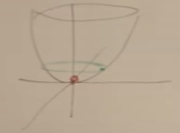
\includegraphics[width=0.8\textwidth]{2-appendix-field-circle}
\end{figure}

Figure \ref{fig:mexican-hat} shows a different potential, with an unstable equilibrium at the origin. This is like a world where the vacuum has a non-zero field. The minimum is a circle centred on the origin: we can set a particle vibrating without expending any energy. If rotation corresponds to charge, we can get a charge without expending energy--a condensate.
\begin{figure}[H]
	\begin{center}
		\caption{Mexican Hat potential}\label{fig:mexican-hat}
		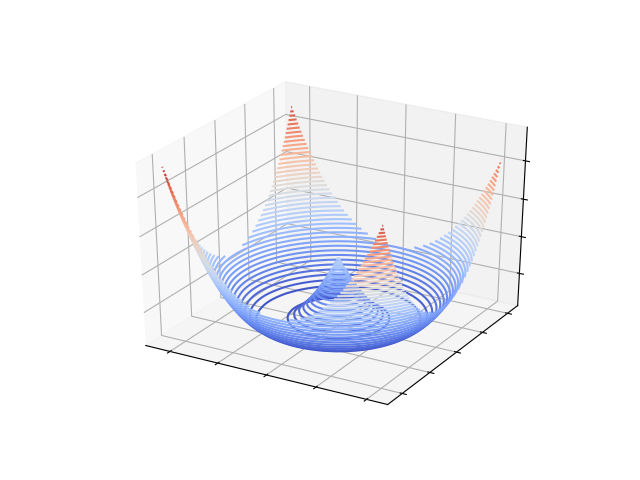
\includegraphics[width=0.6\textwidth]{mexican-hat}
	\end{center}
\end{figure}

True lowest energy should be a stationary state on circle, to avoid kinetic energy. But the uncertainty principle prohibits standing still with zero momentum: if we know that the field is zero, we don't know the velocity. The vacuum must be filled with an uncertain amount of charge.

Imagine that we throw in an extra charge, which displaces vacuum charge by one unit. Charge is uncertain, and we don't notice that we've added or subtracted one! This is part of the weirdness of condensates.

While this isn't true for empty space in the real world, it is exactly what we see with a superconductor!

\section{The Standard Model}

Particles have mass: maximum is Planck Mass - anything heavier would form a black hole. Largest known particle is $\approxeq 10^{-17}$ Planck mass: why so light? To detect a really huge particle we need a humungous accelerator. Maybe there are heavier particles?

I have skipped over list of Fermions and Bosons. They should all be \emph{massless} (see below). In part this explains why masses so small. Figure \ref{fig:sm:processes} depicts some processes from the Standard Model, which are relevant to this Lecture.

\begin{figure}[H]
	\caption{Processes of the Standard Model (not exhaustive)}\label{fig:sm:processes}
	\begin{subfigure}[t]{0.3\textwidth}
		\caption{Charged Fermion emits boson}
		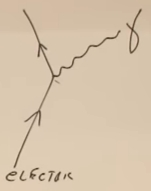
\includegraphics[width=0.9\textwidth]{2-a2-feynman1}
	\end{subfigure}
	\begin{subfigure}[t]{0.3\textwidth}
		\caption{Quark emits gluon}
		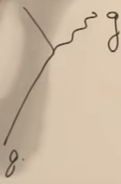
\includegraphics[width=0.9\textwidth]{2-a2-feynman2}
	\end{subfigure}
	\begin{subfigure}[t]{0.3\textwidth}
		\caption{Fermion(even neutrino) emits Z-boson}
		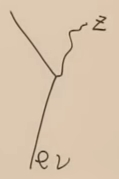
\includegraphics[width=0.9\textwidth]{2-a2-feynman3}
	\end{subfigure}
\end{figure} 

We have a theory to account for the mass of the proton being zero, but it would leave the gluon and Z with zero mass also.

How might fields make different masses for different particles? Figure \ref{fig:2-a2-water-molecule} depicts an analogy, the water molecule. Notice that the mass does not depend on its orientation, because of the symmetry of space. Think of water molecules as particles, $up$ and $down$. In Figure \ref{fig:2-a2-water-molecule-in-field}, switching on the electric field makes the left hand molecules have less energy relative to right hand. We can think of them being two different molecules, "water", say, and "scotch". Since $E=mc^2$, they have different mass. Field exerts no nett force, but affects mass.  

\begin{figure}[H]
	\caption{Analogy: the water molecule and its mass}\label{fig:2-a2-water-molecule}
	\begin{subfigure}[t]{0.4\textwidth}
		\caption{Independent of orientation}
		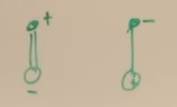
\includegraphics[width=0.9\textwidth]{2-a2-water-molecule}
	\end{subfigure}
	\begin{subfigure}[t]{0.4\textwidth}
		\caption{Depends on orientation relative to field}\label{fig:2-a2-water-molecule-in-field}
		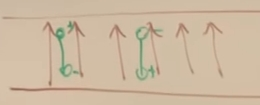
\includegraphics[width=0.9\textwidth]{2-a2-water-molecule-in-field}
	\end{subfigure}
	\begin{subfigure}[t]{\textwidth}
		\caption{Water molecule moving through condensate. Cross indicates that emitted photon is lost in condensate.}\label{fig:2-a2-water-molecule-in-condensate}
		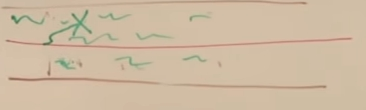
\includegraphics[width=0.9\textwidth]{2-a2-water-molecule-in-condensate}
	\end{subfigure}
\end{figure}

Many printed accounts compare field to molasses. But field doesn't slow particles down! 

Figure \ref{fig:2-a2-water-molecule-in-condensate} depicts the field as a condensate of Bosons, with water molecule moving through it. As molecule moves it is emitting and absorbing photons that are lost in condensate.

\begin{defn}[condensate]
	An indefinite number of particles. In a condensate it doesn't matter whether you put in a particle or take one out.
\end{defn}

Is there any reason why a particle needs the Higgs phenomenon to have a  mass? Figure \ref{fig:2-a2-box-of-radiation} depicts a massless, perfectly reflective box of radiation. Since $E=mc^2$, this box acquires mass. Figure \ref{fig:2-a2-box-of-gluons} depicts the proton as a box of quarks and gluons. Even if the quarks and gluons were massless, the proton would lose only about 1\% of its mass; the rest comes from the kinetic energy of its contents. Protons and black holes don't need the Higgs mechanism. We will concentrate on electrons.

\begin{figure}[H]
	\caption{How to get a mass}
	\begin{subfigure}[t]{0.45\textwidth}
		\caption{A massless, perfectly reflective box of radiation}\label{fig:2-a2-box-of-radiation}
		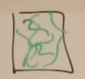
\includegraphics[width=0.9\textwidth]{2-a2-box-of-radiation}
	\end{subfigure}
	\begin{subfigure}[t]{0.45\textwidth}
		\caption{The proton: a box of quarks and gluons}\label{fig:2-a2-box-of-gluons}
		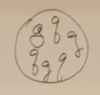
\includegraphics[width=0.9\textwidth]{2-a2-box-of-gluons}
	\end{subfigure}
\end{figure}

\section{The Dirac Electron}

There are two kinds of electrons, right handed and left handed. They can flip, but not if they were travelling at the speed of light (time infinitely slow); in the Dirac theory, mass is the rate at which handedness flips. See Figure \ref{fig:2-a3-flipping-electron}. Figure \ref{fig:2-a3-Z-boson} depicts the Z boson, which can be emitted by electrons or neutrinos. The coupling isn't charge--it is called "weak hypercharge", or, as Prof Susskind says, "zilch". Zilch is like electric charge, but it isn't electric charge. When a particle with zilch accelerates, it emits a Z-boson.

\begin{figure}[H]
	\caption{Electron flipping between left and right}
	\begin{subfigure}[t]{0.65\textwidth}
		\caption{The faster the electron travels, the slower it flips. Probability of jumping is measure of mass}\label{fig:2-a3-flipping-electron}
		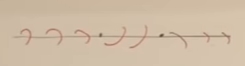
\includegraphics[width=0.9\textwidth]{2-a3-flipping-electron}
	\end{subfigure}
	\begin{subfigure}[t]{0.3\textwidth}
		\caption{Electron emitting Z-boson. }\label{fig:2-a3-Z-boson}
		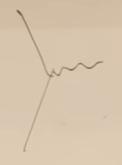
\includegraphics[width=0.9\textwidth]{2-a3-Z-boson}
	\end{subfigure}	
\end{figure} 

Left-handed and right-handed electrons have the same charge but different zilch: LH +1, RH 0. So zilch changes as electron changes from left to right, which is impossible since it is conserved. So the standard model electron has zero mass.

We get around this by introducing the Ziggs boson. This is related to the Mexican Hat, Figure \ref{fig:mexican-hat}, and forms a condensate. It has zilch. Figure \ref{fig:2-a3-zilch} shows an electron exchanging zilch with the condensate via Ziggs bosons. This is the mechanism by which electrons, quarks, and their partners get their mass.

\begin{figure}[H]
	\caption{Spontaneous breaking of chiral symmetry}
	\begin{subfigure}[t]{0.4\textwidth}
		\caption{Spontaneous breaking of chiral symmetry: electron exchanging zilch with the condensate via Ziggs bosons}\label{fig:2-a3-zilch}
		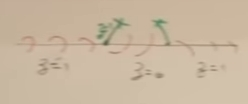
\includegraphics[width=\textwidth]{2-a3-zilch}
	\end{subfigure}
	\begin{subfigure}[t]{0.4\textwidth}
		\caption{Z-boson becoming a Ziggs by exchanging zilch with continuum}\label{fig:2-a3-zilch-Z}
		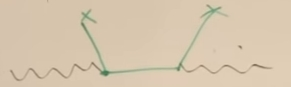
\includegraphics[width=\textwidth]{2-a3-zilch-Z}
	\end{subfigure}
\end{figure}

\section{The Z boson}

How does the Z boson get a mass?

Figure \ref{fig:2-a3-zilch-Z} shows a Z-boson exchanging zilch with the condensate; it oscillates between Z and Ziggs, thereby getting mass. This is known as the Brout-Englert-Higgs phenomenon.

If there were a condensate of electric charge, the proton would have mass, which would be Very Bad.

The Ziggs was discovered in 1980: it is a part of the Z-boson.

\section{The Higgs}

So what is the Higgs? There are two ways to think of it.
\begin{itemize}
	\item Imagine a vibration in the condensate, which makes the particles more and less dense. That is the Higgs.
	\item Imagine particles on Mexican Hat oscillating up and down the potential--Figure \ref{fig:2-a3-higgs1}. This increases and reduces density: it is the Higgs.
\end{itemize}

\begin{figure}[H]
	\caption{Particles on Mexican Hat oscillating up and down the potential}\label{fig:2-a3-higgs1}
	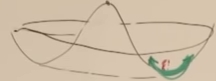
\includegraphics[width=0.8\textwidth]{2-a3-higgs1}
\end{figure}

The Higgs is important because it is the one element of the Standard Model that had not been discovered.

Why was is so hard to discover?

Figure \ref{fig:2-a3-higgs-decay} depicts the decay of the Higgs: heavy particles are favoured. We can read diagram either left to right or right to left. We have been colliding electrons and positrons for a long time, and need very high energy. In addition cross section of reaction is slow.

How about quarks? The usual ones are very light. Lightness of particles made production of Higgs unlikely. Best candidate is the top quark, the heaviest. Use top and antitop. But they aren't easy to find: they decay quickly. We have to make them. Figure \ref{fig:2-a3-gluons} depicts protons colliding at LHC: they contain gluons that make the top quark. 

\begin{figure}[H]
	\caption{How to make a Higgs}
	\begin{subfigure}[t]{0.3\textwidth}
		\caption{Higgs decaying: probability $\propto$ mass of particles produced}\label{fig:2-a3-higgs-decay}
		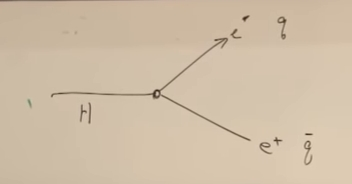
\includegraphics[width=0.8\textwidth]{2-a3-higgs-decay}
	\end{subfigure}
	\begin{subfigure}[t]{0.3\textwidth}
		\caption{Gluons to top to Higgs}\label{fig:2-a3-gluons}
		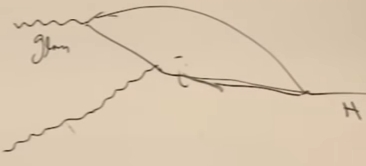
\includegraphics[width=0.8\textwidth]{2-a3-gluons}
	\end{subfigure}
	\begin{subfigure}[t]{0.3\textwidth}
		\caption{More formal version of Figure \ref{fig:2-a3-gluons} }\label{fig:2-a3-higgs-neat}
		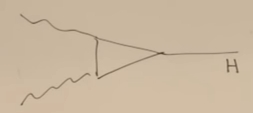
\includegraphics[width=0.8\textwidth]{2-a3-higgs-neat}
	\end{subfigure}
\end{figure}

The near future.

The standard model is essentially correct. Is everything fitting together quantitatively? Figure \ref{fig:2-a3-higgs-neat} provides a hint. We should be able to run this backwards and decay Higgs, but it isn't easy to see gluons. Replace gluons with photons. Higgs can decay into photons. At the time of the lecture, Higgs appears to decay into photons a little too quickly--1.5 times. Maybe something else is going on: maybe some other heavy particle is there. Keep watching. 

\bibliographystyle{unsrt}
\addcontentsline{toc}{section}{Bibliography}
\bibliography{tm}

\end{document}
